\documentclass[12pt]{article}
\usepackage{amsmath}
\usepackage{amsthm}
\usepackage[english]{babel}
\usepackage{float}
\usepackage{graphicx}
\usepackage{amssymb}
\usepackage{hyperref}
\usepackage[utf8]{inputenc}
\usepackage{listings}
\usepackage{pgf, tikz}
\usepackage{xcolor}
\usepackage{geometry}
\usepackage [english]{babel}
\usepackage [autostyle, english = american]{csquotes}
\MakeOuterQuote{"}
\geometry{margin=1in}
\usepackage[utf8]{inputenc}
\newtheorem{theorem}{Theorem}
\newtheorem{example}{Example}
\newtheorem{remark}{Remark}[section]
\newtheorem{definition}{Definition}[section]
\theoremstyle{definition}

% Sensible defaults for lstlistings
\lstset{
  basicstyle=\footnotesize\ttfamily,
  belowcaptionskip=1\baselineskip,
  breaklines=true,
  commentstyle=\bfseries\color{purple!40!black}
  frame=L,
  identifierstyle=\color{blue},
  keywordstyle=\bfseries\color{green!40!black},
  language=python,
  showstringspaces=false,
  stringstyle=\color{orange},
}
\newcommand{\dsep}{\perp \!\!\!\perp}
\title{\vspace{-3cm} Background Draft}
\author{Canyon Foot}


\begin{document}
\maketitle

\section{Introduction}
Bareinboim, Tian, and Pearl's 2014 paper "Recovering from Selection Bias in Causal and Statistical Inference" provides a formulation of selection bias explicitly in terms of causal DAGs and d-separation, making it an especially important resource for developing our study of the topic. In particular, the paper provides graphical conditions (in terms of d-separations) under which a \emph{conditional} distribution $P(y | x)$ can be obtained from a causal graph containing a selection mechanism. However, the content of the paper is highly abstracted and does not attempt to provide real-life cases in which their techniques are useful. For this reason, we will summarize the main results of the paper and interpret them in the context of some realistic examples. 

The paper is broken into three sections, the first two of which are the most substantial and the focus of our attention. The first gives conditions for recovery when only the biased distribution is accessible, the second gives conditions for the case where population level data is available for some variables, and the last gives a brief discussion of recovering causal effects.

\section{A Famous Case of Selection Bias}
One classic example of selection bias sometimes used to introduce the concept is the 1936 presidential election poll  published in an American magazine called The Literary Digest. The election was between Franklin Delano Roosevelt, the democratic incumbent, and Alfred Landon, a republican. The Literary Digest conducted a poll, drawing from their readership and by telephone. The sample size was extremely large, with over 2 million survey respondents. Their prediction, that Landon would comfortably win the election, proved embarrassing. Not only did Landon lose, but he lost in one of the largest electoral landslides in American history:  523 electoral votes went to Roosevelt and 8 went to the Digest's predicted winner. Shortly after, the magazine ceased publication.

The problem was that although their survey had a plenty large sample size, it was non-representative of the population as a whole. Particularly, both being subscribed to The Literary Digest and owning a telephone were more common among more affluent people, and so their survey skewed wealthier than the population as a whole, and therefore underestimated the proportion of voters who would vote for Roosevelt, a candidate with largely working class support. This is no doubt a simplification, but for the moment, let us assume that income was the only variable that was responsible for the non-representative sample, and that this information was collected from respondents as part of the survey. 

One of the important feature of selection bias is that unlike sampling variation, it cannot be reduced with sufficiently large sample sizes. For this reason, in the rest of the paper we will discuss a selection biased joint distribution for this survey, and thereby ignore sample size.

\section{Recovering $P(y|x)$ Without External Data}
In the simplest case, we only have access to a distribution corresponding to a causal graph $G$  with a set of nodes $\mathbf{X}$ equipped with a selection node $S$. This means that we do not have access to the full joint distribution $P(\mathbf{x})$ but rather the conditional joint distribution $P(\mathbf{x} | S = 1)$. This corresponds to the joint distribution of values that are selected to be sampled. So, returning to our election example, our graph would look like:
\begin{center}
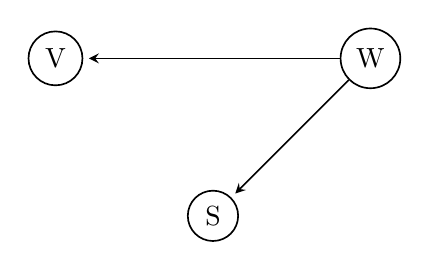
\begin{tikzpicture}[
            > = stealth, % arrow head style
            shorten > = 2pt, % don't touch arrow head to node
            auto,
            node distance = 3cm, % distance between nodes
            semithick % line style
        ]
\node[shape=circle,draw=black] (V) at (0,0) {V};
\node[shape=circle,draw=black] (W) at (4,0) {W};
\node[shape=circle,draw=black] (S) at (2,-2) {S};

 \path [->] (W) edge node[left] {} (S);
 \path [->] (W) edge node[left] {} (V);

\end{tikzpicture}
\end{center}
Where $V$ is a random variable for the candidate a person intends to vote for, $W$ is measures income and $S$ is a binary variable denoting inclusion in the study. Although in practice we would probably like to know $P(v)$, the population level distribution of intended votes, for now we restrict ourselves to $P(v | w)$, the conditional distribution of intended vote given SES. 

In the vein, Bareinboim et al. define \textbf{s-recoverability} as the criterion which must be satisfied for a conditional distribution such as $P(v|w)$ to be obtainable under selection bias. We reproduce their definition exactly and give an explanation of why it makes sense.

\begin{definition}
Given a causal graph $G_s$ augmented with a node $S$ encoding the selection mechanism, the distribution $Q = P(y | \mathbf{x})$ is said to be \textbf{s-recoverable} from selection biased data in $G_s$ if the assumptions embedded in the causal model render $Q$ expressible in terms of the distribution under selection bias $P(\mathbf{v} | S = 1)$. Formally, for every two probability distributions $P_1$ and $P_2$ compatible with $G_s$, $P_1(\mathbf{v} | S = 1) = P_2(\mathbf{v} | S = 1) > 0$ implies $P_1(y | \mathbf{x}) = P_2(y | \mathbf{x})$.
\end{definition}

If we have a selection biased distribution, we have access to a particular joint distribution, $P(\mathbf{v} | S = 1)$ where $\mathbf{V}$ is the set of all nodes other than $S$. So if we are to recover $P(y | \mathbf{x})$ ($\mathbf{X} \subset \mathbf{V}$, $Y \in \mathbf{V}$) we need to express $P(y | \mathbf{x})$ as values derivable from $P(\mathbf{v} | S = 1)$ and the conditional independences implied by the d-separations within the graph. This is what is meant by "if the assumptions embedded in the causal model render $Q$ expressible in terms of the distribution under selection bias $P(\mathbf{v} | S = 1)$", and it is worth exploring why this fairly intuitive formulation is equivalent to the formal definition given in the last sentence.

Consider that the agreement of $P_1$ and $P_2$ on the joint distribution $P(\mathbf{v} | S = 1)$ means that $P_1$ and $P_2$ produce the same observational distribution under selection bias. Therefore, when $P_1(\mathbf{v} | S = 1) = P_2(\mathbf{v} | S = 1) \implies P_1(y | \mathbf{x}) = P_2(y | \mathbf{x})$ we know that no matter the differences between $P_1$ and $P_2$, they must produce the same conditional $P(y|\mathbf{x})$. So, if this is true for every $P_1$, $P_2$, then all distributions consistent with the observational $P(\mathbf{v} | S = 1)$ produce the same $P(y | \mathbf{x})$. 
The first important result of the paper is the following theorem:
\begin{theorem}
The distribution $P(y | \mathbf{x})$ is s-recoverable from $G_s$ if and only if $S \dsep_{G_s} Y | \mathbf{X}$.
\end{theorem}

The proof of $\impliedby$ is quite long, but $\implies$ is easy. 

\begin{proof}
Assume that $S \dsep_{G_s} Y | \mathbf{X}$. Then by the Markov property, $S \dsep Y | X$ and $P(y | \mathbf{x}, S = 1) = P(y | \mathbf{x})$. So the 'recovered' distribution is simply the biased distribution.
\end{proof} 

Clearly this is a useful result since it is easy to test whether two nodes are d-separated by a set. In our application, we can see that $V \dsep_G S | W$, and so $P(v|w) = P(v|w, S = 1)$. So our study gives us direct access to the conditional distribution for candidate preference by income. This is potentially useful but restricted. What if we wish to recover a conditional distribution but do not want to condition on the full separating set? To do so, we will need external measurements.

\section{Recovery With External Data}

Sometimes a researcher will conduct a survey and collect variables on survey participants for which we know the population level distribution. For instance, the US Census collects and publishes data on occupation, race, income, and many other variables from the entire US population. If some of these variables are measured in our selection biased study, this information can be used to recover distributions that would otherwise be unavailable. To elaborate on this topic we will introduce a more complex model of the selection mechanism in our voter poll. In addition to income affecting a person's likelihood of responding to the survey, we will assume that whether a person lives in a city affects both their voter preference and the probability of being included in the survey, independent of income. Then our modified causal graph $G$ would look like this:

\begin{center}
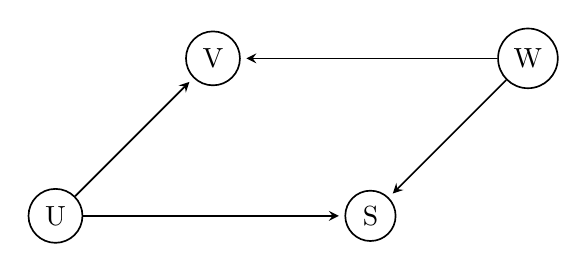
\begin{tikzpicture}[
            > = stealth, % arrow head style
            shorten > = 2pt, % don't touch arrow head to node
            auto,
            node distance = 3cm, % distance between nodes
            semithick % line style
        ]
\node[shape=circle,draw=black] (V) at (0,0) {V};
\node[shape=circle,draw=black] (W) at (4,0) {W};
\node[shape=circle,draw=black] (U) at (-2,-2) {U};
\node[shape=circle,draw=black] (S) at (2,-2) {S};

 \path [->] (W) edge node[left] {} (V);
 \path [->] (U) edge node[left] {} (S);
  \path [->] (W) edge node[left] {} (S);
 \path [->] (U) edge node[left] {} (V);

\end{tikzpicture}
\end{center}

Where $U$ is a binary variable denoting whether the person lives in a city. Under this model, we have a path $S \leftarrow U \rightarrow V$ which is not blocked by $W$. So $S \not \dsep_G Y | X$ and by the previous theorem, we cannot recover $P(v|w)$. Of course, we could recover $P(v | w, u)$ since $S \dsep_G V | \{W,U\}$, but assuming we are still interested in $P(v|w)$, what can be done? 

Well, we could consult the US census and gather the  joint distribution for income and city-living $P(u, w)$. This is what we would call \emph{external data} since it is not affected by the selection mechanism. It turns out that in this case, we can do something. To address this situation, Bareinboim et al.  introduce a revised definition  of s-recoverability which we again reproduce and comment on. 
 
\begin{definition}
Given a causal graph $G_s$ augmented with a node $S$ encoding the selection mechanism, the distribution $Q = P(y | \mathbf{x})$ is said to be \textbf{s-recoverable} from selection bias in $G_s$ with external data over $\mathbf{T} \subseteq \mathbf{V}$ and selection biased data over $\mathbf{M} \subseteq \mathbf{V}$ if the the assumptions embedded in the causal model render $Q$ expressible in terms of the distribution under selection bias $P(\mathbf{m} | S = 1)$ and $P(\mathbf{t})$, both positive. Formally, for every two probability distributions $P_1$ and $P_2$ compatible with $G_s$, if they agree on the available distributions $P_1(\mathbf{v} | S = 1) = P_2(\mathbf{v} | S = 1) > 0$, $P_1(\mathbf{t}) = P_2(\mathbf{t})$ they must agree on the query distribution $P_1(y | \mathbf{x}) = P_2(y | \mathbf{x})$.
\end{definition}

We can see that this definition follows the same structure as the original s-recoverability definition, but is expanded to allow for the use of population level distributions. The paper's second theorem follows directly from this definition.

\begin{theorem}
If there is a set $C \subseteq V$ such that $P(\mathbf{c}, \mathbf{x})$ is measured in the population and $Y \dsep_{G_s} S | \{C,X\}$ then $P(y | \mathbf{x})$ is s-recoverable as

$$P(y | \mathbf{x}) = \sum_{\mathbf{c}} P(y | \mathbf{x}, \mathbf{c}, S = 1)P(\mathbf{c} | \mathbf{x})$$
\end{theorem}

The theorem is a straightforward application of the law of total probability.
\begin{proof}
By assumption, we have the external distribution $P(\mathbf{c}, \mathbf{x})$ and therefore $P(\mathbf{c} | \mathbf{x})$, and as usual we have $P(\mathbf{v} | S =  1)$. So can apply the law of total probability and the conditional independence $Y \dsep S | \{C,X\}$ to write:

$$P(y | \mathbf{x}) = \sum_{\mathbf{c}} P(y | \mathbf{x}, \mathbf{c}) P(\mathbf{c} | \mathbf{x}) = \sum_{\mathbf{c}} P(y | \mathbf{x}, \mathbf{c}, S = 1) P(\mathbf{c} | \mathbf{x})$$

\end{proof}

Therefore, if we wish to recover $P(v | w)$ when living in a city is affects selection, we can do so using the external data $P(u | w)$.

\section{A Useful Extension}
As we have seen, Bareinboim et al. is focused on the recovery of conditional distributions, i.e. $P(v|w)$. However, we would often like to have the unconditional distribution $P(v)$. Although it is only mentioned obliquely at the end of the second section, the results they prove give a simple condition for when $P(v)$ is recoverable using external data. In both sections we have seen that $P(v|w)$ was recoverable. Then, assuming that we have the external data for $P(w)$, we can use the law of total probability to write:

$$P(v) = \sum_{w} P(v|w)P(w).$$

More generally, we can formulate this result as a theorem, although it is not listed as such in the paper.

\begin{theorem}
If there exists a set $\mathbf{X} \subseteq V$ such that $P(y|\mathbf{x})$ is s-recoverable and $P(\mathbf{x})$ is available externally, then $P(y)$ is recoverable as $P(y) = \sum_{\mathbf{x}} P(y|\mathbf{x})P(\mathbf{x})$.
\end{theorem}
\end{document}
 